%===================================================================================
\subsection{CU28 Ver estadisticas de avances de las tareas}
{
\justify
\color{blue}{\textbf{Objetivo}}
}

%------------------------------------------------------------------
\justify
Permite al Lider de proyecto visualizar los diagramas con los reportes de avances registrados por el mismo lider así como de los colaboradores del proyecto.
%------------------------------------------------------------------
{
\justify
\color{blue}{\textbf{Diseño}}
}
%-------------------------------------------------------------------------------
\justify
En la figura \ref{fig:IU28} se muestra la pantalla, en donde permite al Lider de proyecto visualizar los diagramas con los reportes de avances registrados por el mismo lider así como de los colaboradores del proyecto..

\begin{figure}[htb]
\centering
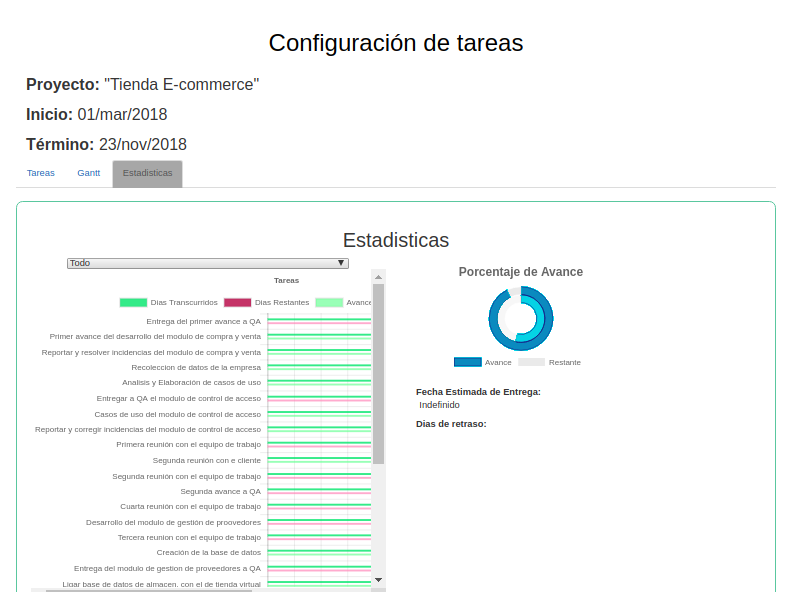
\includegraphics[width=0.8\textwidth]{./images/cu28-ver-estadisticas-avances-tareas.png}
\caption{Ver estadisticas de avances de las tareas.} \label{fig:IU28}
\end{figure}